\documentclass[10pt]{article}
\usepackage{graphicx,amsmath,sidecap,subfigure,comment,amssymb}    % needed for including graphics e.g. EPS, PS
%\usepackage[hidelinks]{hyperref}
\usepackage[table,xcdraw]{xcolor}
%\hypersetup{colorlinks=true}
\usepackage{color}
\usepackage{amsmath,amsthm,amssymb}
\usepackage{gensymb}
\newcommand{\packagename}{\textbf{ncpaprop}}

\usepackage{fancyref}

\usepackage[justification=centering]{caption}
\topmargin -1.5cm        % read Lamport p.163
\oddsidemargin -0.04cm   % read Lamport p.163
\evensidemargin -0.04cm  % same as oddsidemargin but for left-hand pages
\textwidth 16.59cm
\textheight 21.94cm 
%\pagestyle{empty}       % Uncomment if you don't want page numbers
\parskip 5pt           % sets spacing between paragraphs
%\renewcommand{\baselinestretch}{1.5} % Uncomment for 1.5 spacing between lines
%\parindent 40pt		 % sets leading space for paragraphs
\parindent 0.25 in

%\setlength{\parskip}{1em}

\usepackage[margin=1in]{geometry}

\def\deriv#1{\frac{d}{d #1}}
\def\derivs#1#2{\frac{d #1}{d #2}}
\def\parderiv#1{\frac{\partial}{\partial #1}}
\def\parderivs#1#2{\frac{\partial #1}{\partial #2}}
\def\secparderiv#1{\frac{\partial^2}{\partial #1^2}}
\def\secparderivs#1#2{\frac{\partial^2 #1}{\partial #2^2}}

\newcommand{\version}{2.1.0}

\begin{document}

%\input cover_page.tex\clearpage

\vspace*{-50pt}

\includegraphics[width=230pt]{figs/logos/color_logo_UTTR.pdf}
\hspace*{65pt}

\includegraphics[width=150pt]{figs/logos/UM_logo.png}
\vspace*{50pt}


\vspace*{0.05\textheight}

\begin{center}

\begin{Huge} \underline{\textbf{ncpaprop \version}} \end{Huge} 

\vspace*{0.025\textheight} 

\begin{Large}
\underline{NCPA Infrasound Propagation Modeling Package}
\end{Large} 

\vspace*{0.06\textheight}

\textsl{Contributions from: Roger Waxler, Claus Hetzer, Jelle Assink, Doru Velea}

\vspace*{0.02\textheight}

\textsl{Technical coordination: Roger Waxler}

\end{center}

\vspace*{0.06\textheight}

\begin{center}
\raisebox{10pt}{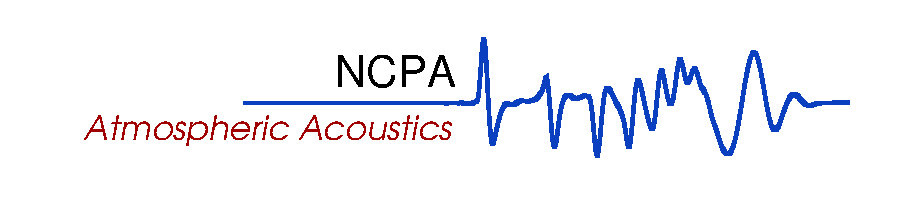
\includegraphics[height=40pt]{figs/logos/noct_logo_2.pdf}}

\includegraphics[height=60pt]{figs/logos/NCPA-Logo-Crest.pdf}
\quad
\raisebox{10pt}{
\includegraphics[height=40pt]{figs/logos/knmi_logo.png}}

\end{center}

\vspace*{\fill}

\noindent\makebox[\linewidth]{\rule{\linewidth}{0.4pt}}

\noindent Roger Waxler, Claus Hetzer, Jelle Assink, and Doru Velea. (2021). https://github.com/chetzer-ncpa/ncpaprop-release: NCPAprop v2.1.0 (v2.1.0). Zenodo. https://doi.org/10.5281/zenodo.5562713

%\vfill
\clearpage
\input legalize.tex

\vspace*{20pt}

%\input acknowledgements.tex
\clearpage
\tableofcontents
\clearpage

\input sections/introduction.tex
\clearpage
\input sections/installation.tex
\clearpage
\input sections/running_code_in_general.tex
\clearpage
\input sections/modess.tex
\clearpage
\input sections/wmod.tex
\clearpage
%\input sections/cmodess.tex
%\clearpage
\input sections/modbb.tex
\clearpage
%\input sections/rdmodess.tex
%\clearpage
%\input sections/pade_pe.tex
%\clearpage
\input sections/ePape.tex
\clearpage
%\input sections/raytrace.tex
%\clearpage
%\input sections/nl_raytrace.tex

\clearpage
\bibliography{ncpaprop}
\bibliographystyle{plain}

\end{document}


.........................
